%!TEX root = ../main.tex

\section{Gaussian Splatting}\label{sec:GS}

\subsubsection{3D Gaussian Splatting}\label{sec:3DGS}


\begin{figure}[htbp]
  \centering
  \includegraphics[width=0.9\textwidth]{figure/40_prelim/3dgs_pipeline.png}
  \caption{
    Gaussian Splattingのパイプライン。
    \cite{Kerbl2023ToG_3DGS}より引用。
    }
    \label{fig:3dgs_pipeline}
\end{figure}

\begin{figure}[htbp]
  \centering
  \includegraphics[width=0.6\textwidth]{figure/40_prelim/nerf_vs_3dgs.png}
  \caption{
    Gaussian SplattingとNeRFとレンダリング方式の違い。
    \cite{Chen2024_3DGS-Survey}より引用。
    (a) NeRFのレンダリング方式。
    (b) 3DGSのレンダリング方式。
    NeRFでは各レイに沿ってサンプリングするため、計算コストが大きいが、GSではラスタライズによる高速なレンダリングを実現する。
    これはGPUの描画パイプラインを効果的に流用する。ラスタライズにより3D空間のGaussianを2D画像平面に投影することを`Splatting'と表現している。
    }
    \label{fig:nerf_vs_3dgs_rendering}
\end{figure}

\missingfigure{NeRFと3DGSの分類図。レンダリング速度と、データサイズの2Dプロット。Barronさんのレクチャー動画から。学習速度も入れれば、2次元に収まらない。。2個いるかな? できれば、MVSとかも含めて示せればいい。それだったら表が美しい}

3D Gaussian Splatting (3DGS) は、新規視点合成において最先端(SOTA)の結果を達成している近年の手法である \parencite{Kerbl2023ToG_3DGS}。
その特徴は、フォトリアリスティックかつ高忠実度な3次元シーンのキャプチャ能力、高速な学習時間、そしてリアルタイムレンダリングにある。
明示的な(Explicit)3次元表現である3DGSは、Visual-SLAM \parencite{Yan2024CVPR_GS-SLAM,Zheng2025CVPR_WildGS-SLAM,Matsuki2024CVPR_GaussianSplattingSLAM}、アバター生成 \parencite{Moreau2024CVPR_HumanGaussianSplatting,Shao2024CVPR_GaussianAvatar}、フィードフォワード型3次元再構成 \parencite{Chen2024ECCV_MVSplatting} など、幅広いタスクへの適用に成功している。
その可能性はさらに広がり、衛星画像からの数値表層モデル(DSM)生成 \parencite{Aira2025CVPR_EOGS}、自動運転、そして水中3次元再構成 \parencite{li20243DV_watersplatting} といった様々な実世界アプリケーションへと拡張されている。
\fix{自動運転}

\begin{figure}[htbp]
  \centering
  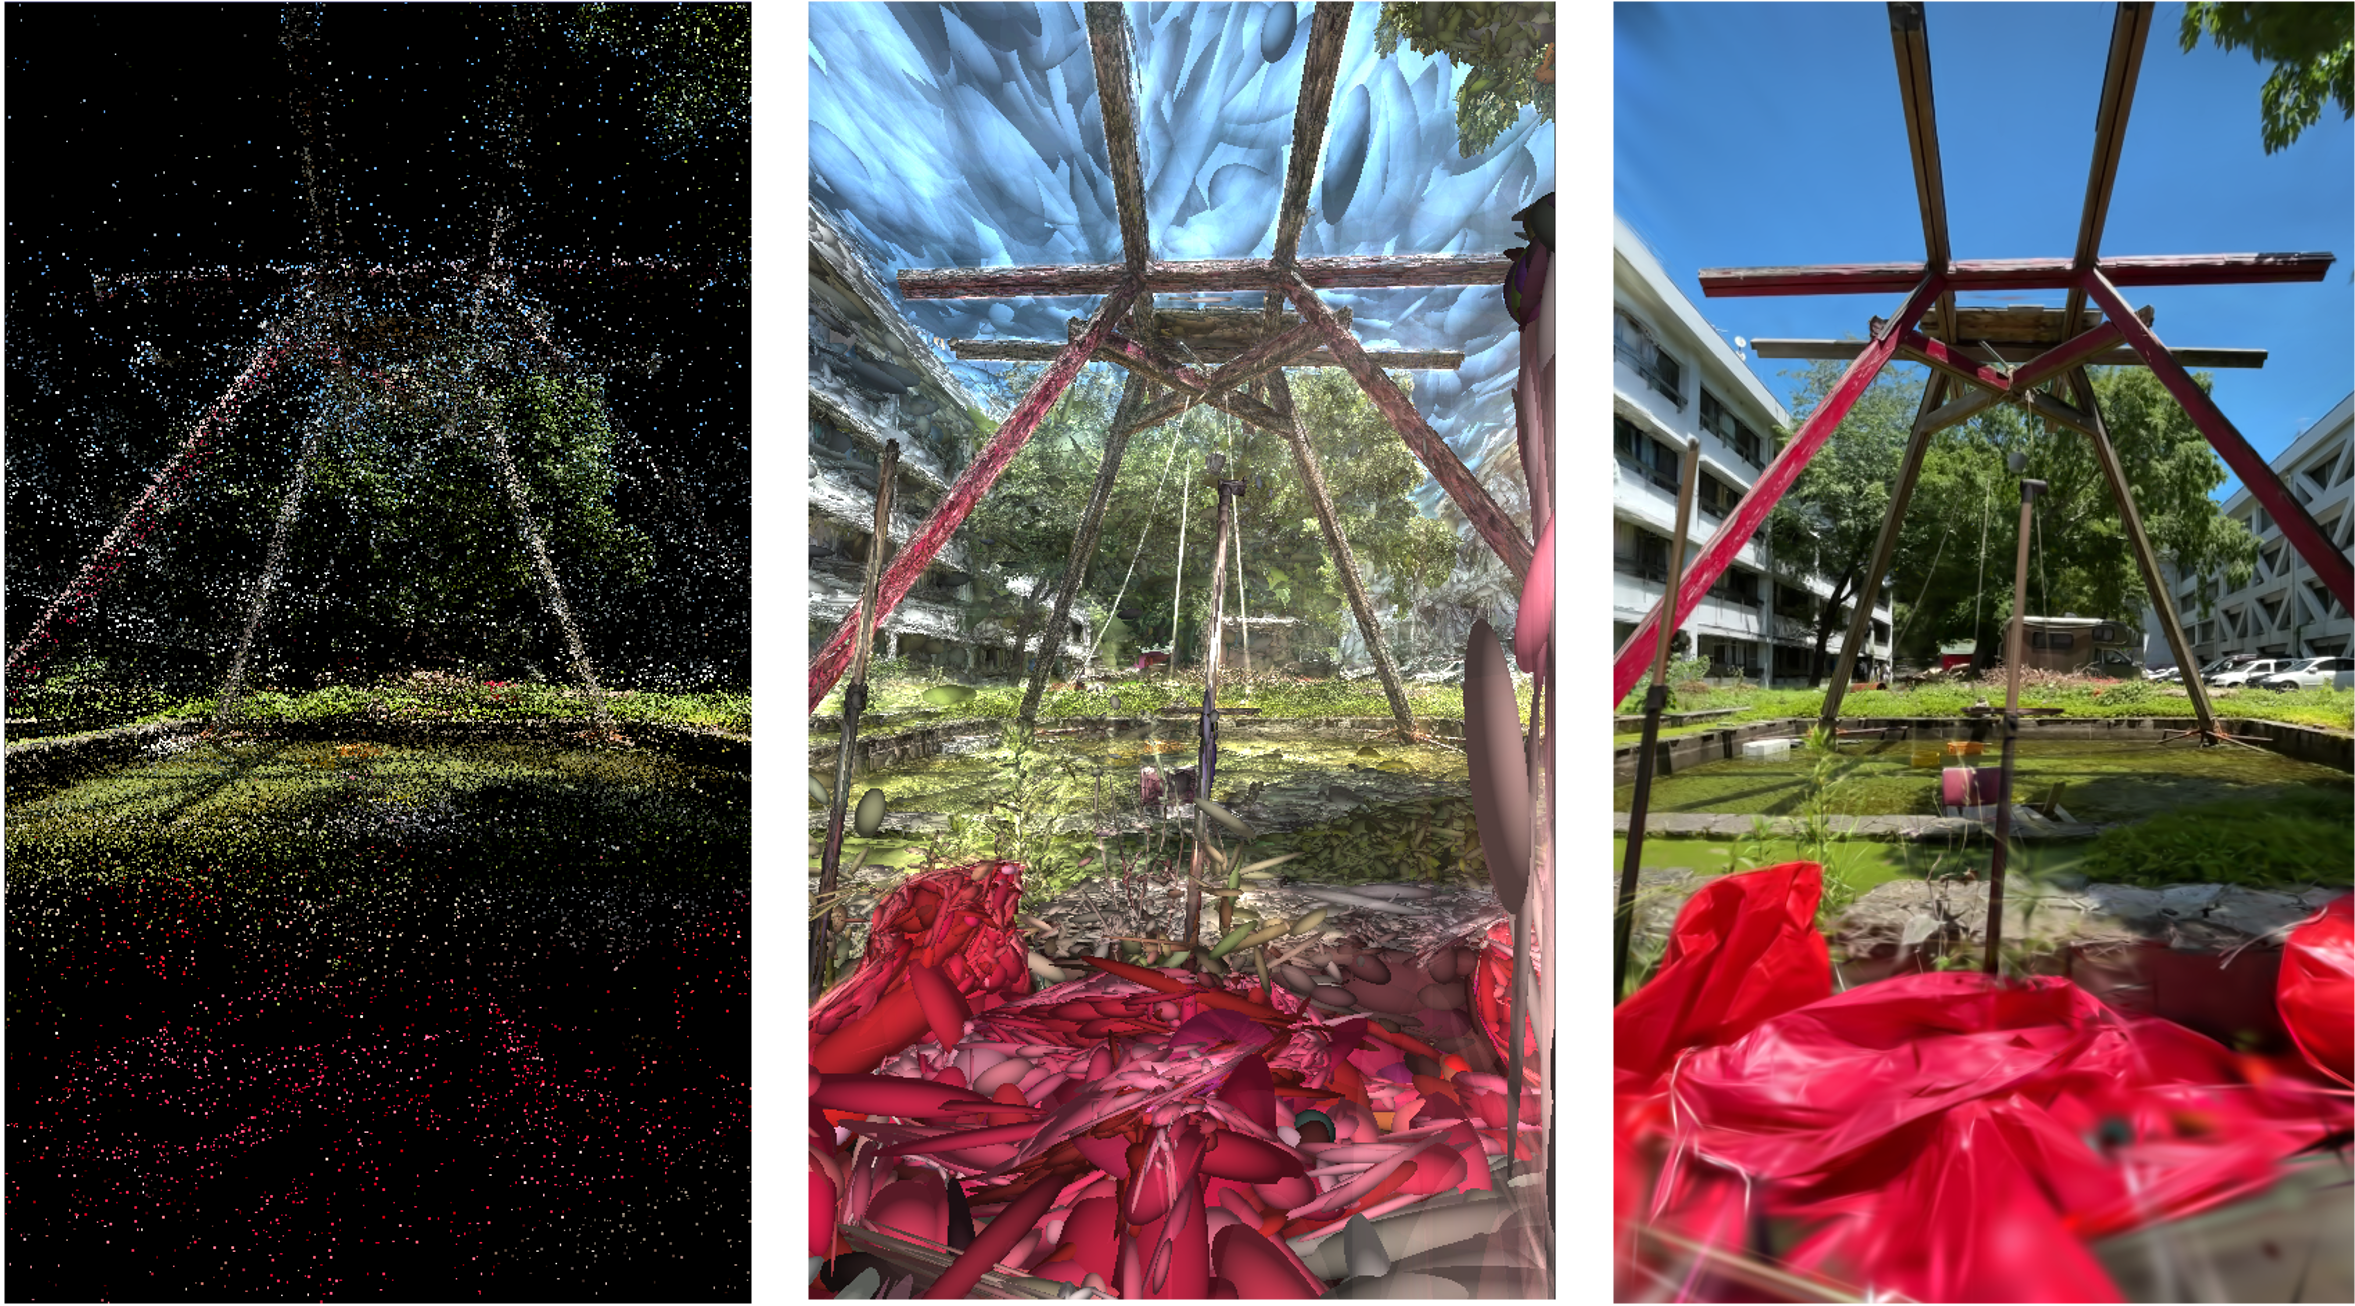
\includegraphics[width=0.7\textwidth]{figure/40_prelim/compare_pc-elip-render.png}
  \caption{
    点群と楕円体のレンダリング結果の比較。
    (a) 点群のレンダリング結果。
    (b) 楕円体のレンダリング結果。
    (c) 最終的な3DGSのアルファブレンディングによるレンダリング結果。
    }
    \label{fig:compare_pc-elip-render}
\end{figure}

3DGSのパイプラインは主に、レンダリングを行うフォワードパスと、最適化を行うバックワードパスの2つの段階で構成される。
フォワードパスでは、3次元ガウス分布(3D Gaussians)の集合を、ラスタライズにより画像平面に投影することで画像を合成する。
各ガウス分布は、
中心位置 $\bm{p} \in \mathbb{R}^3$、
不透明度 $\alpha \in [0, 1]$、
球面調和関数(SH)によって表現される視点依存の色係数 $\bm{c}(\bm{p}, \bm{t}_i) \in \mathbb{R}^{3}$、
および3次元共分散行列 $\bm{\Sigma}^{\mathrm{3D}} \in \mathbb{R}^{3 \times 3}$ 
という、最適化可能なパラメータセットによって定義される。
これらのパラメータは、カメラパラメータを得る際に用いられるSfMで副次的に得られる粗点群を用い初期化される(\cref{fig:3dgs_pipeline}A)。
共分散行列 $\bm{\Sigma}^{\mathrm{3D}}$ は、スケーリングベクトル $\bm{s} \in \mathbb{R}^3$ から構成されるスケーリング対角行列 $\bm{S} \in \mathbb{R}^{3 \times 3}$ と、回転クォータニオン(回転行列 $\bm{R} \in SO(3)$ として表現)を用いて以下のように構成される:
\begin{equation}\label{eq:3dgs-sigma_RssR}
  \bm{\Sigma}^{\mathrm{3D}} = \bm{R} \bm{S} \bm{S}^\top \bm{R}^\top
\end{equation}
点 $\bm{x} \in \mathbb{R}^3$ に対する対応する非正規化ガウス分布関数は以下で与えられる:
\begin{equation}\label{eq:3dgs-G(x)}
  G(\bm{x}) = 
    \exp \left( -\frac{1}{2} (\bm{x} - \bm{p})^T \left({\bm{\Sigma}^{3D}}\right)^{-1} (\bm{x} - \bm{p}) \right)
\end{equation}
フォワードパスにおいて、あるカメラ視点からの画像をレンダリングするために、これらのガウス分布はまず外部パラメータ行列 $[\bm{W} | \bm{t}]$ を用いてワールド座標系からカメラ座標系へと変換される。
ガウス分布の中心位置 $\bm{p}$ と3次元共分散行列は以下のように更新される:
\begin{align*}
  &\bm{p}_\mathrm{cam} = \bm{W}\bm{p} + \bm{t} \\
  &\bm{\Sigma}^{3D}_\mathrm{cam} = \bm{W} \bm{\Sigma}^{3D} \bm{W}^\top
\end{align*} 
ここで、$\bm{W}_\mathrm{view} \in \mathbb{R}^{3 \times 3}$ は視点回転行列、
$\bm{t} \in \mathbb{R}^3$ は平行移動ベクトルである。
\cite{Zwicker2001_EWA-volume-splatting} の提案した射影手法に従い、カメラ空間における3次元共分散行列 $\Sigma_{cam}^{3D}$ は2次元画像平面へと射影される。
これは透視投影の一次近似(アフィン近似)のヤコビ行列 $\bm{J}$ を用いて行われ、2次元共分散行列 $\bm{\Sigma}^{\mathrm{2D}}$ が得られる:
\begin{equation}\label{eq:3dgs-affine-projection}
\Sigma^\mathrm{2D} = \bm{J} \Sigma^{\mathrm{3D}}_\mathrm{cam} \bm{J}^\top
\end{equation}
各ピクセルの最終的なRGB値 $\bm{\Gamma} \in \mathbb{R}^{3}$ は、射影されたガウス分布をアルファブレンディングすることでレンダリングされる。
ピクセルと重なるガウス分布の集合は、まず深度に基づいて手前から奥へとソートされ、視点依存色が以下のように累積される:
\begin{align}\label{eq:3dgs-alpha-blending}
  \bm{\Gamma}(\bm{x}) = \sum_{k=1}^{K} \bm{c}_k \alpha^{\text{pixel}}_k \prod_{j=1}^{k-1} (1-\alpha^{\text{pixel}}_j) \\
  \quad \text{where} \quad \alpha^{\text{pixel}}_k = \alpha_k G_k^{\mathrm{2D}} \notag
\end{align}
ここで、$k$ はピクセルに重なる整列されたガウス分布の集合のインデックスである。

バックワードパスでは、最適化により測光誤差(Photometric loss)を最小化する。
これは $\mathcal{L}_1 (\Gamma, \Gamma_{gt})$ 損失と D-SSIM 損失 $\mathcal{L}_\mathrm{D-SSIM} (\Gamma, \Gamma_{gt})$ \parencite{Zhou2004_SSIM} の加重和である:
\begin{equation}\label{eq:loss-function}
  \mathcal{L} = (1 - \lambda) \mathcal{L}_1 + \lambda \mathcal{L}_\mathrm{D-SSIM}
\end{equation}
したがって、最適化問題は以下のように定式化される:
\begin{equation}\label{eq:optimization}
  \underset{p, R, s, c, \alpha}{\textrm{argmin}} \quad \mathcal{L} = \mathcal{L}(\bm{\Gamma}, \bm{\Gamma_{gt}}) 
\end{equation}
これらの定式化により、パイプライン全体が完全微分可能となり、パラメータ $\Theta = \{\bm{p}, \bm{R}, \bm{s}, \bm{c}, \alpha\}$ はAdamを用いた勾配降下法\parencite{Adam}によって最適化可能となる。
(\cref{fig:3dgs_pipeline}B)

これらの勾配降下法のみでは、特に観測視点が少ない箇所(Few Shot Area)などで、シーンの適切な一貫性に欠ける局所最適解に陥りやすい。
これを解決するために3DGSではAdaptive Density Control(ADC)というヒューリスティックな手法が導入されている。
あるGaussianに関して、その2D平面や3D空間における位置に対する誤差勾配$\frac{\partial \mathcal{L}}{\partial \bm{p}}$が大きい場合、そのGaussianは幾何的な誤差の大きいものであるという推察に基づいて
分割(Split)、複製(Clone)、消去(Prune)のいずれかの操作を行う。
位置誤差勾配がある閾値を超え、さらにシーンに対してGaussianが大きい場合は分割、小さい場合は複製を行う。
また、不透明度$\alpha$が小さいGaussianも消去する。
効果的にシーンに寄与しないGaussianを削除するため、一定のイテレーションごとにシーンのGaussianの不透明度を一様に小さいものにリセットすることで、その後不透明度が向上しないGaussianを削除できるようにする。
\note{MCMCの説明も。?。これらのヒューリスティックスはデータセットや初期値に対して依存するため、それを克服するようなMCMCといった手法も考案されている。}

\begin{figure}[htbp]
  \centering
  \includegraphics[width=0.6\textwidth]{figure/40_prelim/3dgs_adc.png}
  \caption{
    Adaptive Density Control(ADC)の操作。
    \cite{Kerbl2023ToG_3DGS}より引用。
    Gaussianに流れる位置誤差勾配が大きい場合、サイズが小さいGaussianに対しては、複製、サイズが大きいGaussianに対しては、分割を行うことで、適切なサイズのGaussianでシーンを満たす。
    }
    \label{fig:3dgs_adc}
\end{figure}


\begin{center}
  \begin{minipage}{0.8\linewidth}
    \begin{algorithm}[H]\label{alg:3dgs-adc}
      \caption{
        Novel 3DGS\cite{Kerbl2023ToG_3DGS}における密度最適化アルゴリズム。
        \cite{Grubert2025VISAPP_improve-ADC}より引用。
        }
      \SetAlgoLined
      \DontPrintSemicolon
      
      \textbf{Data:} Scene of Gaussians $G$ \\
      \For{$G_k \in G$}{
          \Comment{Densification}
          \If{$\tau_k \geq T_{grad}$}{
              \If{$\max(s_k) > P_{dense} \cdot e_{scene}$}{
                  splitGaussian($G_k$)\;
              }
              \Else{
                  cloneGaussian($G_k$)\;
              }
          }
          
          \Comment{Opacity Pruning}
          \If{$\alpha_k < \alpha_{min}$}{
              pruneGaussian($G_k$)\;
          }
          
          \Comment{Size Pruning}
          \If{$\max(s_k) > 0.1 \cdot e_{scene}$}{
              pruneGaussian($G_k$)\;
          }
      }
    \end{algorithm}
  \end{minipage}
\end{center}

ここで、
$\tau_k$ は2次元位置誤差勾配の平均値、
$P_{dense}$ は密度最適化のハイパーパラメータ、
$T_{grad}$ は位置誤差勾配の閾値ハイパーパラメータ、
$e_{scene}$ はシーンの範囲、
$\alpha_{min}$ は最小不透明度ハイパーパラメータである。


% Adam \parencite{Adam} を用いた~ と言っていたがこれは、Implplementationで言及すること
その最適化に要する学習時間は、30kのイテレーションによって1時間以内となり、当時NVSのSotaであったMip-NeRF360 \parencite{Barron2022CVPR_Mip-NeRF360} に比較して10倍以上の高速化を達成した。
加えて、Ray-Tracingに比較し、既存のGPU描画パイプラインの性能を引き出すTile-Basedレンダリングによって、100 fps以上のリアルタイムレンダリングを実現したことで、インタラクティブなSceneの可視化が可能となった\cref{fig:nerf_vs_3dgs_rendering}。
このプロセスを通じて得られた3次元ガウス分布の集合は、3次元シーンを高忠実度で捉えることができる。


しかし、このパイプライン全体はピンホールカメラモデルと透視投影に依存しており、光が直線的に進むことを根本的な前提としている。
この前提は、空気と水の境界での屈折が幾何学的矛盾を引き起こすような複数の媒質が介在する環境においては成立しない。
この制限にもかかわらず、3DGSの明示的な3次元表現は、屈折の法則を数学的に定式化し、シーン表現の幾何学的パラメータそのものに直接適用することが可能とする。
一方で、3DGSではラスタライズによってレンダリングされるため、レイトレーシングのように容易に屈折の影響をモデル化することができない、という困難も生じる。


\subsection{2D Gaussian Splatting}\label{sec:2DGS}
2D Gaussian Splatting(2DGS) \parencite{Huang2024SIGGRAPH_2DGS}は、Photometricな一貫性に特化した3DGSに対し、幾何的な一貫性を向上させることを目的とした派生手法である。
3次元シーンで観測されるRadianceは、環境光が物体表面で反射したものから観測されるという前提から、3次元シーンの各Gaussianは物体表面に整列して配置されることを目指すMVSなどのGeometric Reconstructionの一種とも言える。

2DGSの3DGSとの違いは、主に以下の3点である:
\begin{itemize}
  \item 平らな2次元ガウス分布(Surfel)プリミティブによる3次元シーン表現
  \item 正確な透視投影(Perspective-accurate)による、2D Gaussian集合の2次元画像平面への射影
  \item 幾何的な整合性を高める正則化の導入
\end{itemize}

2DGSにおいて、シーンは平らな2次元ガウス分布(Surfel)(2D-oriented planar Gaussian disks)の集合として表現される。
つまり、3DGSに比較し、スケーリングベクトル $\bm{s}$のうち最小の成分が0と表現したSurfelとして表現し、
2DGSのプリミティブは、中心位置$\bm{p}_k$、主方向ベクトル$\bm{t}_u$と$\bm{t}_v$、および対応するスケーリングベクトル$\bm{s} = (s_u, s_v)$によって表現される。
(回転行列$\bm{R}_k$、不透明度$\alpha_k$と視線依存色$\bm{c}_k$は3DGSと同様である。)

% レイと第 $k$ プリミティブ平面との交点 $\bm{p}_{inter}$ をローカル座標系へ変換した変位ベクトルを $\bm{u}$ とすると、$\alpha_i$ は以下のように定義される。

% \begin{equation}
%     \alpha_i = o_i \exp\left( -\frac{1}{2} \bm{u}^\top \bm{\Sigma}_{2D}^{-1} \bm{u} \right)
% \end{equation}

% ここで、$o_i$ は学習可能な不透明度パラメータ、$\bm{\Sigma}_{2D}$ は2次元スケーリングと回転行列から構成される局所的な分散行列である。

% \subsection{蓄積アルファ (\texttt{render\_alphas})}
% \textbf{型:} $[..., C, H, W, 1]$

% レイに沿った総不透明度であり、物理的にはレイが物体によって遮蔽された確率を表す。これは最終的な透過率 $T_{final}$ の補数となる。

% \begin{equation}
%     A(\mathbf{r}) = \sum_{i \in \mathcal{N}} \alpha_i T_i = 1 - T_{final} = 1 - \prod_{i=1}^{N} (1 - \alpha_i)
% \end{equation}

% \subsection{ボリューム法線 (\texttt{render\_normals})}
% \textbf{型:} $[..., C, H, W, 3]$

% 2DGSが「幾何学的に正確」であるための核心的な項である。各2次元ガウス円盤の固有法線 $\bm{n}_i$ を、色情報と同様の重みでブレンディングしたものである。

% \begin{equation}
%     \bm{n}_{vol}(\bm{r}) = \sum_{i \in \mathcal{N}} (\bm{R}_i \cdot \bm{z}_{local}) \alpha_i T_i
% \end{equation}

% ここで $\bm{R}_i$ はクォータニオンから導出される回転行列、$\bm{z}_{local} = (0,0,1)^\top$ はローカル座標系における法線ベクトルである。この $\bm{n}_{vol}$ は、後述する表面法線との整合性を取る正則化(Normal Consistency Loss)に使用される。

% \subsection{表面法線 (\texttt{surf\_normals})}
% \textbf{型:} $[..., C, H, W, 3]$

% レンダリングされた深度マップの幾何学的勾配から算出される法線であり、「見かけ上の形状」を表す。まず、期待値深度(Expected Depth) $D(u,v)$ を計算する。

% \begin{equation}
%     D(u, v) = \sum_{i \in \mathcal{N}} t_i \alpha_i T_i
% \end{equation}

% ここで $t_i$ はカメラ原点から交点までの距離である。$\bm{n}_{surf}$ は画像空間における勾配のクロス積として近似される。

% \begin{equation}
%     \bm{n}_{surf} \propto \frac{\partial D}{\partial u} \times \frac{\partial D}{\partial v}
% \end{equation}

% \subsection{歪み (\texttt{render\_distort})}
% \textbf{型:} $[..., C, H, W, 1]$

% Mip-NeRF 360で提案されたDistortion LossのL1変種である。レイ上の密度分布が局所的に集中(=明確な表面が存在)することを奨励する。

% \begin{equation}
%     \mathcal{L}_{dist}(\bm{r}) = \sum_{i, j} w_i w_j |t_i - t_j| + \frac{1}{3} \sum_i w_i^2 s_i
% \end{equation}
% (ただし実装上は計算効率化のため、上記式の簡易版が用いられる場合がある)

% \subsection{中央値深度 (\texttt{render\_median})}
% \textbf{型:} $[..., C, H, W, 1]$

% 累積透過率が閾値0.5に達した地点の深度。期待値深度におけるエッジ付近のアーティファクト(Flying Pixels)を抑制し、TSDF Fusion等によるメッシュ再構成において堅牢な結果を提供する。

% \begin{equation}
%     t_{median} = \mathop{\mathrm{argmin}}_t \left| \int_{0}^{t} \alpha(s)T(s) \mathrm{d}s - 0.5 \right|
% \end{equation}

% \section{実装上の設計指針 (Engineering Advice)}

% Google Researchの実装経験に基づき、安定したパイプライン構築のための重要な指針を以下に示す。

% \subsection{Ray-Plane Intersectionの特異点処理}
% 視線ベクトル $\bm{d}$ と平面法線 $\bm{n}_i$ が直交に近い場合(Grazing Angle)、交点計算は数値的に不安定となる。CUDAカーネル内では、内積値に対するハードクリッピングを推奨する。

% \begin{equation}
%     \text{if } |\bm{d} \cdot \bm{n}_i| < \epsilon \quad (\text{e.g., } \epsilon=0.05), \quad \text{discard intersection.}
% \end{equation}

% \subsection{幾何再構成のための深度モード}
% メッシュ抽出を目的とする場合、\texttt{depth\_mode}の選択は重要である。浮遊ノイズの少ない高品質なメッシュを得るためには、\texttt{render\_median} の出力を信頼するか、あるいは正則化項を含んだ \texttt{RGB+ED} モードでの学習結果を用いることが望ましい。また、微分可能レンダリングにおいて \texttt{surf\_normals} を利用する際は、計算グラフの切断(detach)を適切に管理する必要がある。






具体的には、3D空間内の2次元ガウス分布は、ローカルな接平面 $(u, v)$ 上で定義され、その幾何学的形状は同次変換行列 $\bm{H} \in \mathbb{R}^{4 \times 4}$ を用いて以下のようにパラメータ化される \parencite{Huang2024SIGGRAPH_2DGS}。

\begin{equation}\label{eq:2dgs-plane-def}
  \bm{H} = 
  \begin{bmatrix}
    s_u \bm{t}_u & s_v \bm{t}_v & \bm{0} & \bm{p}_k \\
    0 & 0 & 0 & 1
  \end{bmatrix}
\end{equation}

ここで、ローカル座標 $\bm{u} = (u, v)$ におけるガウス分布の強度は、標準的な2次元ガウス関数として定義される。
\begin{equation}
  G(\bm{u}) = \exp\left( - \frac{u^2 + v^2}{2} \right)
\end{equation}

\subsubsection{Perspective-Accurate Splatting via Ray-Splat Intersection}
3DGSが採用しているアフィン近似による投影は、ガウス分布の中心から離れるにつれて近似誤差が増大し、視点によって深度が不整合になるという問題がある。
これに対し2DGSは、視線レイ(Ray)と2次元平面(Splat)の交差判定(Ray-Splat Intersection)を明示的に計算することで、正しい透視投影を実現する。

スクリーン空間上のピクセル座標 $\bm{x} = (x, y)$ を通る視線レイは、3次元空間において直交する2つの平面(x-planeとy-plane)の交線として定義できる。
これを同次座標系の4次元平面ベクトル $\bm{h}_x = (-1, 0, 0, x)^\top, \bm{h}_y = (0, -1, 0, y)^\top$ として表現し、これらをワールド空間からスクリーン空間への変換行列 $\bm{W}$ と、先述のローカル変換行列 $\bm{H}$ を用いてガウス分布のローカル座標系へ逆変換する。
ここで、平面の変換には逆転置行列 $(\bm{W}\bm{H})^{-\top}$ を用いる必要があるが、これにより明示的な逆行列計算を回避し、数値的な安定性を保つことができる。

\begin{equation}\label{eq:2dgs-h-transform}
  \bm{h}_u = (\bm{W}\bm{H})^\top \bm{h}_x, \quad \bm{h}_v = (\bm{W}\bm{H})^\top \bm{h}_y
\end{equation}

この変換された平面 $\bm{h}_u, \bm{h}_v$ と、ローカル平面上の点 $(u, v, 1, 1)^\top$ との内積が0になるという条件から、交差点 $\bm{u}(\bm{x})$ を以下の閉形式で高速に求めることができる。

\begin{equation}\label{eq:2dgs-intersection}
  \bm{u}(\bm{x}) = \frac{1}{\bm{h}_u^3 \bm{h}_v^4 - \bm{h}_u^4 \bm{h}_v^3} 
  \begin{pmatrix}
    \bm{h}_u^2 \bm{h}_v^4 - \bm{h}_u^4 \bm{h}_v^2 \\
    \bm{h}_u^4 \bm{h}_v^1 - \bm{h}_u^1 \bm{h}_v^4
  \end{pmatrix}
\end{equation}
ここで $\bm{h}^i$ はベクトルの第 $i$ 成分を表す。これにより得られた $\bm{u}(\bm{x})$ を用いて $G(\bm{u}(\bm{x}))$ を評価することで、正確なレンダリングが可能となる。

また、2DGS特有の問題として、視線が円盤に対して平行に近い角度(Slanted viewpoint)になった際に、スクリーン上で線分に退化し、勾配消失やエイリアシングを引き起こす現象がある。
これを防ぐため、2DGSではローパスフィルタ $\sigma$ を導入し、スクリーン空間での最小サイズを保証する以下のクリッピング処理を行う。
\begin{equation}
  \hat{G}(\bm{x}) = \max \left\{ G(\bm{u}(\bm{x})), G\left( \frac{\bm{x} - \bm{c}}{\sigma} \right) \right\}
\end{equation}
この処理は実装上、最適化の安定性を確保するために極めて重要である。
\note{ローパスフィルタまでは説明しなくても良い。(3DGSでも説明していないから)。MipSplatting説明しないといけない}

\subsubsection{Regularization for Geometric Consistency}
2DGSはSurfel表現を持つが、単なるPhotometric lossのみでは、3次元再構成特有の不定性によりノイズの多い表面形状に収束してしまう傾向がある。
そこで、幾何学的精度を向上させるために\cite{Barron2022CVPR_Mip-NeRF360}で提案された2つ正則化項をGSフレームワークに導入している。

一つ目は \textbf{Depth Distortion Loss} ($\mathcal{L}_d$) である。
3DGSのボリュームレンダリングは、レイ上の交点間の距離を考慮しないため、ガウス分布が前後に散らばるアーティファクトが生じやすい。
2DGSでは、レイ上の交差点深度 $z_i$ とブレンディング重み $\omega_i$ を用いて、寄与の高いガウス分布同士の深度距離を最小化するように制約をかける。

\missingfigure{依然、木津川で再構成した際のアーティストを示す}
\begin{figure}[htbp]
  \centering
  \includegraphics[width=0.7\textwidth]{figure/40_prelim/2dgs_regulatization.png}
  \caption{
    2DGSの正則化項の効果。
    左から順に、入力画像、法線整合性正則化なしの表面法線、深度歪み正則化なしの表面法線、そして両方の正則化を適用した2DGSの結果である。
    法線整合性正則化を適用しない場合、表面の法線方向にノイズが生じる。
    一方、深度歪み正則化を省略すると、法線マップがぼやけたものとなる。
    両方の正則化を併用することで、鋭く滑らかな表面形状を正確に再構成できている。
    }
    \label{fig:2dgs_regulatization}
\end{figure}



\begin{equation}
  \mathcal{L}_d = \sum_{i, j} \omega_i \omega_j |z_i - z_j|
\end{equation}

二つ目は \textbf{Normal Consistency Loss} ($\mathcal{L}_n$) である。
2DGSのプリミティブは自身が法線ベクトル $\bm{n}_i = \bm{t}_u \times \bm{t}_v$ を持っている。
ここで $\times$ はベクトルの外積演算を表す。
この明示的な法線と、レンダリングされた深度マップから推定される法線 $\bm{N}$(深度の勾配 $\nabla \bm{D}$ から算出)との整合性を取ることで、滑らかな表面再構成を強制する。

\begin{equation}
  \mathcal{L}_n = \sum_{i} \omega_i (1 - \bm{n}_i^\top \bm{N})
\end{equation}

最終的な損失関数は、3DGSのPhotometric lossに加え、これらの正則化項を加重和したものである。
これらの幾何学的制約により、2DGSはNoiseの少ない詳細なメッシュ抽出が可能となり、かつ3DGSと同等のレンダリング速度と画質を維持している。

\note{メッシュの抽出にはTSDF Fusionを用いている。}
